\documentclass[10pt, titlepage, oneside, a4paper]{article}
\usepackage[T1]{fontenc}
\usepackage[utf8]{inputenc}
\usepackage[swedish]{babel}
\usepackage{amssymb, graphicx, fancyhdr}
\usepackage{hyperref}
\usepackage{pgf, tikz}
\usepackage{pgfplots}
\usepackage{listings}
\usepackage{color}
\usepackage{amsmath}
\usepackage{mathtools}
\addtolength{\textheight}{20mm}
\addtolength{\voffset}{-5mm}
\renewcommand{\sectionmark}[1]{\markleft{#1}}

\newcommand{\Section}[1]{\section{#1}\vspace{-8pt}}
\newcommand{\Subsection}[1]{\vspace{-4pt}\subsection{#1}\vspace{-8pt}}
\newcommand{\Subsubsection}[1]{\vspace{-4pt}\subsubsection{#1}\vspace{-8pt}}


\def\typeofdoc{Laborationsrapport}
\def\course{F0004T}
\def\pretitle{Laboration 1}
\def\title{Svängningstid av svängande svängningar}
\def\username{magbjr-3}
\def\domain{@student.ltu.se}
\def\email{\username{}@student.ltu.se}
\def\group{Grupp 10}
\def\graders{Magnus Frediksson}
\def\university{Luleå Tekniska Universitet}


\def\fullpath{\raisebox{1pt}{$\scriptstyle \sim$}\username/\path}


\begin{document}
	\begin{titlepage}
		\thispagestyle{empty}
		\begin{large}
			\begin{tabular}{@{}p{\textwidth}@{}}
				\textbf{\university\hfill\today}\\
				\textbf{\typeofdoc} \\
			\end{tabular}
		\end{large}
		\vspace{10mm}
		\begin{center}
			\LARGE{\pretitle} \\
			\huge{\textbf{\course}}\\
			\vspace{10mm}
			\LARGE{\title}\\
			\vspace{15mm}
			\begin{large}
				\begin{tabular}{l|ll}
                    \textbf{\group} & \textbf{Namn} & \textbf{E-mail}\\
                    \hline
                    & \texttt{Anton Eriksson}   & \texttt{eriano-4\domain}       \\
                    & \texttt{Eric Öhman}   & \texttt{erihma-3\domain}       \\
                    & \texttt{Magnus Björk}   & \texttt{magbjr-3\domain}       \\
				\end{tabular}
			\end{large}
			\vfill
			\large{\textbf{Handledare}}\\
			\mbox{\large{\graders}}
		\end{center}
	\end{titlepage}


	\lfoot{\footnotesize{\group}}
	\rfoot{\footnotesize{\today}}
	\lhead{\sc\footnotesize\title}
	\rhead{\nouppercase{\sc\footnotesize\leftmark}}
	\pagestyle{fancy}
	\renewcommand{\headrulewidth}{0.2pt}
	\renewcommand{\footrulewidth}{0.2pt}

	\pagenumbering{roman}
    \begin{abstract}
        Bacon ipsum dolor amet short ribs chicken porchetta meatball jerky landjaeger ball tip. Biltong frankfurter ham hock, strip steak pork belly flank salami pig pancetta sirloin boudin ball tip swine. Rump picanha drumstick salami pancetta ham hock strip steak. Beef ribs porchetta shank, meatloaf swine chicken pork. Rump drumstick prosciutto sirloin.

Pork belly capicola ball tip, shankle biltong porchetta hamburger tail. Capicola pork chop rump brisket, ham tongue corned beef prosciutto kielbasa pork short ribs flank frankfurter shankle. Kielbasa meatball ribeye spare ribs. Leberkas shank prosciutto spare ribs brisket porchetta pancetta pork boudin beef tail capicola fatback pork loin pig. Hamburger short loin tongue pastrami cupim ham shankle meatball drumstick kielbasa ball tip pork cow. Tongue bresaola ball tip rump filet mignon short ribs, alcatra tri-tip pig leberkas jowl. Fatback bacon jerky frankfurter.

Doner filet mignon turducken beef pork loin cow meatball venison spare ribs bacon. Hamburger sausage ribeye turkey short ribs, venison landjaeger doner bacon cupim frankfurter salami meatball beef ribs pork chop. Landjaeger sausage venison t-bone shankle. Hamburger swine chicken pastrami bresaola, pork chop brisket cupim tail tenderloin turkey cow meatloaf.

Brisket venison pork chop pig salami tongue ball tip pork belly. Pork fatback short ribs pork chop sirloin bacon doner brisket turducken ham hock. Chicken ribeye fatback beef ribs, landjaeger pork chop bresaola ball tip. Strip steak jowl frankfurter fatback alcatra.

Kielbasa cow short loin jowl doner jerky corned beef short ribs. Meatloaf t-bone short loin short ribs cupim boudin cow chuck swine alcatra fatback. Tongue pork belly prosciutto filet mignon pork. Pork loin landjaeger tri-tip shank corned beef doner meatloaf ham swine strip steak jowl boudin venison chicken. Biltong frankfurter kevin, bacon turkey meatball filet mignon cupim turducken rump tenderloin hamburger beef short loin landjaeger. Doner salami pig jowl.
    \end{abstract}
    
    \tableofcontents
	
	\newpage

	\pagenumbering{arabic}

	\setlength{\parindent}{10pt}
	\setlength{\parskip}{10pt}
	

    
	\section{Inledning}
	\section{Metod}
	\section{Resultat}
    \begin{center}
        \begin{figure}[h]
            \centering
            \includegraphics[scale=.5]{../png/height.png}
            \caption{Svängningstid beroende på tjocklek.}
            \label{height}
        \end{figure}
        \begin{figure}
            \centering
            \includegraphics[scale=.5]{../png/length.png}
            \caption{Svängningstid beroende på längd.}
            \label{length}
        \end{figure}
        \begin{figure}
            \centering
            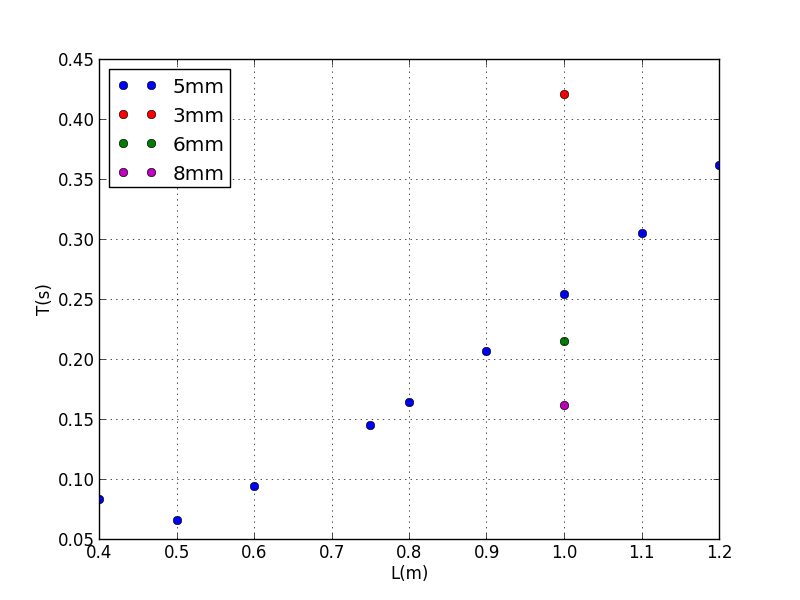
\includegraphics[scale=.5]{../png/plot.png}
            \caption{Svängningstid beroende på material.}
            \label{material}
        \end{figure}
        \begin{figure}
            \centering
            \includegraphics[scale=.5]{../png/ln_t_ln_l.png}
            \caption{linearisering}
            \label{linearisering}
        \end{figure}
    \end{center}

    \begin{table}
        \caption{Undersökning av längd.}
        \begin{center}
            \begin{tabular}{cccc}
                \hline
                Tid (s) & Längd (m) & Höjd (m) & Bredd (m)\\
                \hline
                0.362 & 1.200 & 0.005 & 0.020\\
                0.305 & 1.100 & 0.005 & 0.020\\
                0.254 & 1.000 & 0.005 & 0.020\\
                0.207 & 0.900 & 0.005 & 0.020\\
                0.164 & 0.800 & 0.005 & 0.020\\
                0.145 & 0.750 & 0.005 & 0.020\\
                0.094 & 0.600 & 0.005 & 0.020\\
                0.066 & 0.500 & 0.005 & 0.020\\
                0.083 & 0.400 & 0.005 & 0.020\\
            \end{tabular}
        \end{center}
    \end{table}

    \begin{table}
        \caption{Undersökning av längd.}
        \begin{center}
            \begin{tabular}{cccc}
                \hline
                Tid (s) & Längd (m) & Höjd (m) & Bredd (m)\\
                \hline
                0.255 & 1.000 & 0.005 & 0.020\\
                0.259 & 1.000 & 0.005 & 0.025\\
                0.250 & 1.000 & 0.005 & 0.030\\
                0.259 & 1.000 & 0.005 & 0.040\\
            \end{tabular}
        \end{center}
    \end{table}

    \begin{table}
        \caption{Undersökning av längd.}
        \begin{center}
            \begin{tabular}{cccc}
                \hline
                Tid (s) & Längd (m) & Höjd (m) & Bredd (m)\\
                \hline
                0.421 & 1.000 & 0.003 & 0.020\\
                0.254 & 1.000 & 0.005 & 0.020\\
                0.215 & 1.000 & 0.006 & 0.020\\
                0.162 & 1.000 & 0.008 & 0.020\\
            \end{tabular}
        \end{center}
    \end{table}

	\section{Analys}
    \section{Diskussion}


\end{document}

